%% General definitions
\documentclass{article} %% Determines the general format.
\usepackage{a4wide} %% paper size: A4.
\usepackage[utf8]{inputenc} %% This file is written in UTF-8.
%% Some editors on Windows cannot save files in UTF-8.
%% If there is a problem with special characters not showing up
%% correctly, try switching "utf8" to "latin1" (ISO 8859-1).
\usepackage[T1]{fontenc} %% Format of hte resulting PDF file.
\usepackage{fancyhdr} %% Package to create a header on each page.
\usepackage{lastpage} %% Used for "Page X of Y" in the header.
											%% For this to work, you have to call pdflatex twice.
\usepackage{enumerate} %% Used to change the style of enumerations (see below).

\usepackage{amssymb} %% Definitions for math symbols.
\usepackage{amsmath} %% Definitions for math symbols.
\usepackage{amsthm}
\usepackage{braket}
\usepackage{graphicx}
\usepackage{float}

\usepackage{tikz}  %% Pagacke to create graphics (graphs, automata, etc.)
\usetikzlibrary{automata} %% Tikz library to draw automata
\usetikzlibrary{arrows}   %% Tikz library for nicer arrow heads


%% Left side of header
\lhead{\course\\\semester\\Exercise \homeworkNumber}
%% Right side of header
\rhead{\authorname\\Page \thepage\ of \pageref{LastPage}}
%% Height of header
\usepackage[headheight=36pt]{geometry}
%% Page style that uses the header
\pagestyle{fancy}

\newcommand{\authorname}{Nico Bachmann\\Ruben Hutter}
\newcommand{\semester}{Spring semester 2023}
\newcommand{\course}{Theory of Computer Science}
\newcommand{\homeworkNumber}{3}


\begin{document}

\section*{Exercise \homeworkNumber.1}
\begin{enumerate}[(a)]
	\item
	A possible derivation of the word "abaabaaba" is:
	$$
	1 \; (aSa) \to 2 \; (abSba) \to 1 \; (abaSaba) \to 1 \; (abaaSaaba) \to 4 \; (abaabaaba)
	$$
	
	\item
	$\mathcal{L}(G)$ is the definition of a Palindrome. The word can always be read either forward or
	backward and you get the same result.
	
	\item
	The Grammar that represents a representation of binary trees is:
	$$
	G = \left \langle \set{S}, \; \set{[, \circ, \square, ]}, \; R, \; S \right \rangle
	$$
	with R:
	\begin{enumerate}[1)]
		\item
		$S \to \square$
		
		\item
		$S \to [S \circ S]$
		
	\end{enumerate}
	
\end{enumerate}

\clearpage

\section*{Exercise \homeworkNumber.2}
\begin{enumerate}[(a)]
	\item
	To check if $G_1 = \left \langle \set{S, X, Y}, \set{a, b}, R_1, S \right \rangle$ is a regular
	language we rewrite the rules set. In a first step we eliminate the start variable from the
	right-hand side of $R_1$ and in a second step we eliminate forbidden occurrences of $\epsilon$ and
	obtain:
	$$
	R_1' = \set{S \to aX, \; S \to aS', \; S \to \epsilon, \; S' \to a, \; S' \to aX, \; S' \to aS', \;
	X \to ba, \; X \to bX}
	$$
	So we see that this is a regular grammar and therefore of Type-3, and because of Type-3 also of
	Type-$i \text{ for } i < 3$.

	\item
	To-Do

\end{enumerate}

\clearpage

\section*{Exercise \homeworkNumber.3}


\clearpage

\section*{Exercise \homeworkNumber.4}
\begin{figure}[h]
		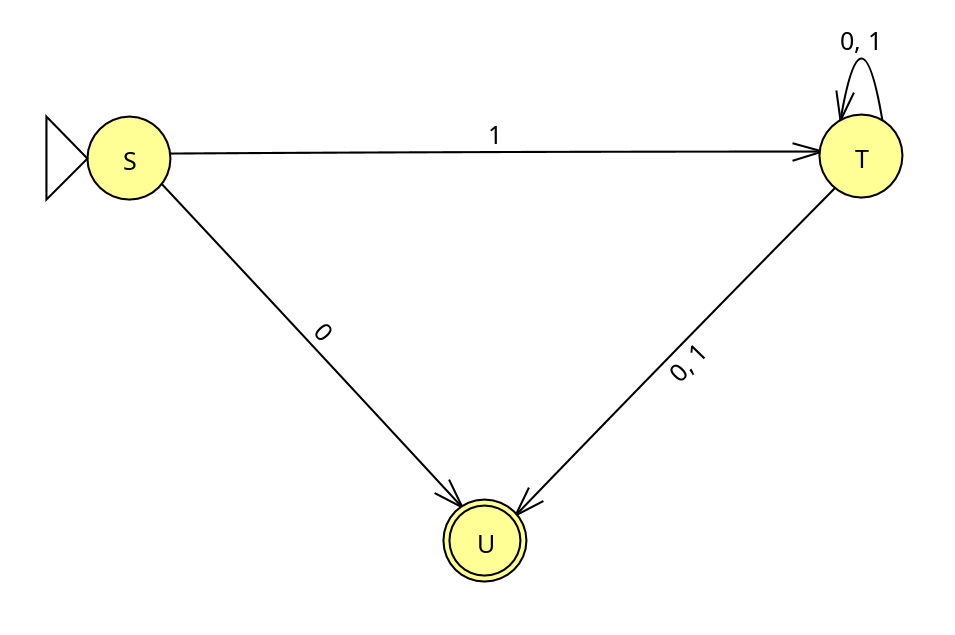
\includegraphics[width=\linewidth]{ex4.png}
		\centering
		\caption{NFA for $G$}
	\end{figure}

\section*{Exercise \homeworkNumber.5}
\end{document}
